\chapter{Methodology}\label{ch:methodology}
This chapter describes the methodology behind \benchmark and the design decisions that were made in order to address the research question. It explains how the benchmark evaluates \ac{rl} agents operating in power grids, which aspects of agent performance are measured and how these are aggregated into a final score. Additionally, the chapter provides a recommended protocol for setting up and conducting an evaluation with \benchmark.

\section{Benchmark Structure}\label{sec:benchmark-structure}
Figure \ref{fig:tool-steps} shows a simplified version of the benchmark's steps. The tool receives a \ac{rl} agent as input. This agent is then run in multiple scenarios, each of which yields a score. These scores are then aggregated to create a final score, which is the benchmark's output for the given agent. The score consists of multiple metrics and categories, as explained in depth in Section \ref{sec:metrics-eval}.

\begin{figure}[htp] 
    \centering
    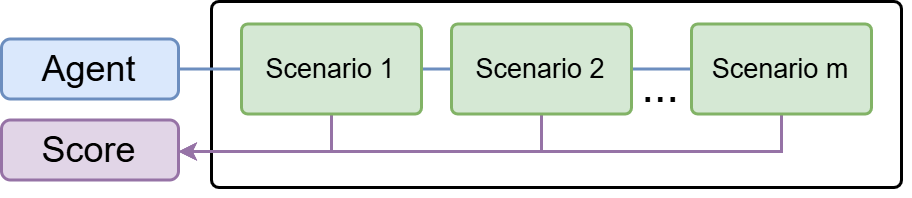
\includegraphics[width=0.6\textwidth]{images/methodology/tool_steps_reduced.png}
    \caption{Summarised benchmark process of \benchmark evaluating one agent}
    \label{fig:tool-steps} 
\end{figure}

In \benchmark, a \textbf{scenario} is defined as a five-tuple 
\[(\text{Network}, \text{Profile}, \text{Modifications}, \text{Eval}_{idx}, ep_{len})\]
where network is the topology description of a power grid, profile shows the changes of the generators and loads in the network over a range of time, and modifications are changes over the grid, e.g. scaling of specific generators or reducing the capacity of a line (explained more in depth in Section \ref{ssec:implementation-grid-mod}). $\text{Eval}_{idx}$ is the set of starting indices to use for a single scenario run $i\in\text{Eval}_{idx}$. Each agent starts running from index $i$ until $i + ep_{len}$ for each run. Thus $ep_{len}$ defines the episode length. This tuple design was chosen to make each scenario reproducible and to differentiate between scenarios. If any component of this tuple is changed, the resulting scenario has a different scope and complexity. Altering the network can result in a new grid topology that differs greatly in size and complexity. This affects the difficulty of stabilising the power grid during the simulation. When the profile or grid modification is changed, power generation and consumption might become much easier or harder for the \ac{rl} agent to manage. Furthermore, the score is influenced by the length of the episode. The longer the episode, the more difficult it is to maintain a stable grid. Additionally, the starting indices impact the difficulty of maintaining grid stability in a scenario. For example, energy consumption is higher in the evening than during the day because most people are at home using electricity.

\benchmark also enables the user to use custom agents. Those agents must potentially be trained before they can be evaluated. Hence, \ac{rl} agents get the following six-tuple
\[(\text{Network}, \text{Profile}, \text{Modifications}, \text{Train}_{idx}, \text{Eval}_{idx}, ep_{len})\]
which additionally has the $\text{Train}_{idx}$ information. $\text{Train}_{idx}$ and $\text{Eval}_{idx}$ define the indices to start training or evaluation from, respectively. They do not have any overlapping indices, as the agent must be trained on different indices compared to the evaluation indices. This tests the agent's performance on unknown grid states. Although the agent is trained on a scenario, it is evaluated on each evaluation index separately.
The used technologies and the implementation of these steps are explained further in Chapter \ref{ch:implementation}.



\section{Metrics and Evaluation}\label{sec:metrics-eval}
To evaluate the quality of the agent, data from each run is collected in the form of different grid metrics. These metrics are then aggregated into a final score that is the output of the benchmark. Each metric can be classified into one category that the benchmark focusses on.

\subsection{Metric Categories}\label{ssec:metric-categories}
The metrics are categorised into five different groups, which are demonstrated in Figure \ref{fig:categories-bm}. These categories are used to calculate the score of a run, which will be explained further in Section \ref{ssec:score-calc}. Each category contains a variety of metrics for evaluating the agent's performance. Table \ref{tab:metric_categories} in the appendix lists all the metrics in each category.

The metrics in the \textbf{overload mitigation} category measure how well the agent avoids line overloads. Examples of these metrics include the timesteps without overloads and the number of overloaded transmission lines. Depending on the settings chosen by the user, the overload mitigation metrics can also include $N-1$ overload metrics. This setting is discussed further in Section \ref{sec:int-processes}.
In the \textbf{voltage violation mitigation} category, metrics determine how well the agent mitigates bus voltage violations. These include, for example, metrics that measure the maximum or mean percentage of voltage deviation from the nominal values at the buses in a timestep. 
The \textbf{survival} category contains only one metric that indicates how many timesteps the agent kept the power grid in a stable, converged state. A state is considered converged when the power flow equations can be successfully solved. Convergence does not necessarily imply operational safety, hence the inclusion of voltage violations, overloads and other operational metrics in \benchmark. 
The \textbf{costs} category focuses on metrics that determine operational costs, such as frequency of actions on substations, power losses, and load shedding (where loads receive insufficient or no electricity). 
Finally, the \textbf{computational performance} category evaluates runtime, as well as CPU and memory usage. Some metrics have two parts, one measuring the average value of the metric over the course of the episode, and the other measuring the worst observed value. In Section \ref{sec:metrics-description} in the appendix there is a more detailed explanation for each metric, and which metrics are measured by their average and worst value. 

\begin{figure}[htp]
    \centering
    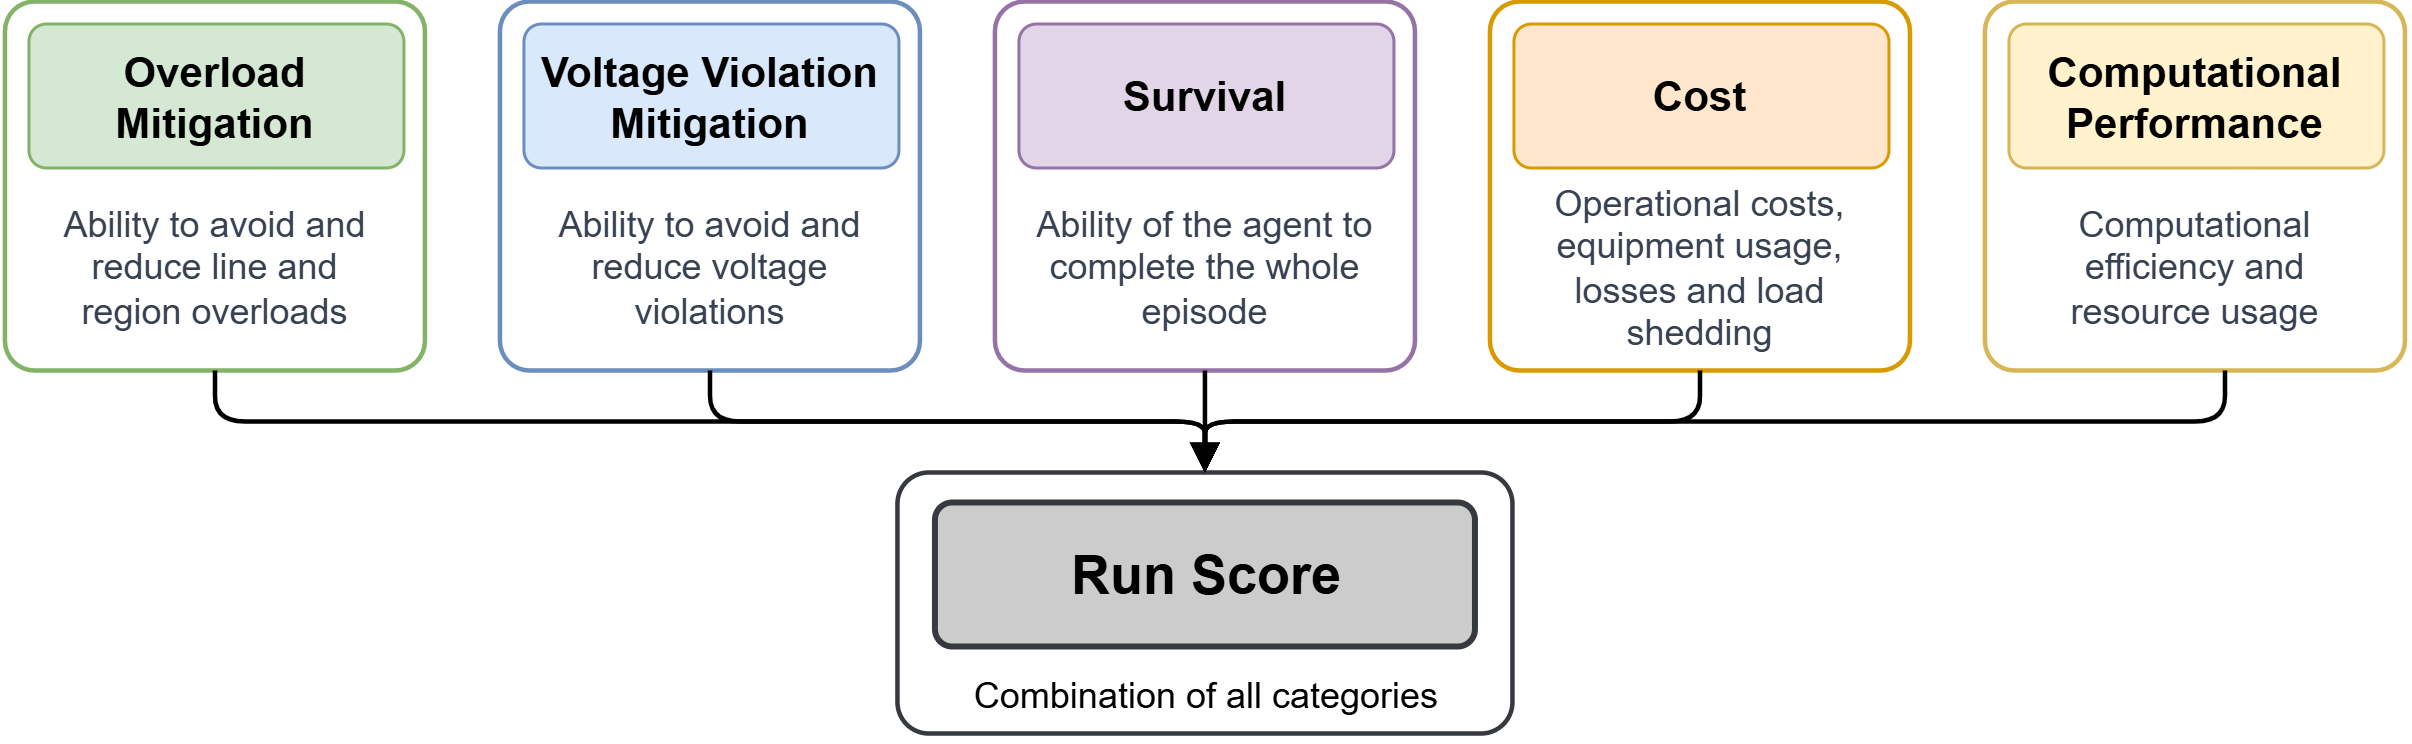
\includegraphics[width=0.99\textwidth]{images/methodology/benchmark_categories.png} 
    \caption{Evaluation categories of \benchmark that form the run score}
    \label{fig:categories-bm} 
\end{figure}

\subsection{Score Calculation}\label{ssec:score-calc}
Each metric has a different numerical range. Therefore, the scoring function normalises every metric value to a score between 0 and 100, where 0 represents the worst score and 100 represents the best score. This is done by defining a worst value \(x_{\mathrm{worst}}\) and a best value \(x_{\mathrm{best}}\) for each metric. Values between these two bounds are mapped linearly to the interval \([0, 100]\), while values outside the bounds are clipped to either 0 or 100.

Equations \eqref{eq:linear_metric_score_increasing} and \eqref{eq:linear_metric_score_decreasing} define the scoring function for the two possible cases. Equation \eqref{eq:linear_metric_score_increasing} applies to metrics where larger values are better, while Equation \eqref{eq:linear_metric_score_decreasing} applies to metrics where smaller values are better. For example, for the number of survived timesteps in an episode, the best value is the episode length \(ep_{\mathrm{len}}\), while the worst value is 0. In contrast, for the total number of timesteps with voltage violations, this relation is reversed. The best value is 0, while the worst value is \(ep_{\mathrm{len}}\). Section \ref{sec:metrics-description} in the appendix contains the exact values of \(x_{\mathrm{worst}}\) and \(x_{\mathrm{best}}\) for each metric.

\begin{equation}
s(x) =
\begin{cases}
0, & x \leq x_{\mathrm{worst}}, \\[4pt]
100 \cdot \dfrac{x - x_{\mathrm{worst}}}{x_{\mathrm{best}} - x_{\mathrm{worst}}},
& x_{\mathrm{worst}} < x < x_{\mathrm{best}}, \\[8pt]
100, & x \geq x_{\mathrm{best}},
\end{cases}
\qquad
\text{for } x_{\mathrm{worst}} < x_{\mathrm{best}}.
\label{eq:linear_metric_score_increasing}
\end{equation}

\begin{equation}
s(x) =
\begin{cases}
100, & x \leq x_{\mathrm{best}}, \\[4pt]
100 \cdot \dfrac{x_{\mathrm{worst}} - x}{x_{\mathrm{worst}} - x_{\mathrm{best}}},
& x_{\mathrm{best}} < x < x_{\mathrm{worst}}, \\[8pt]
0, & x \geq x_{\mathrm{worst}},
\end{cases}
\qquad
\text{for } x_{\mathrm{worst}} > x_{\mathrm{best}}.
\label{eq:linear_metric_score_decreasing}
\end{equation}

Each metric and category has a weight. These weights are used to emphasise specific metrics or categories, or to allow users to omit those that are not important for their goals. For example, the computational performance category might not be as significant as other categories if a lot of resources are available and the user's goal is not to optimise resource usage. 
These weights are used to calculate an aggregated score for each run. Equation \eqref{eq:run_score} shows these calculations. For each category $c \in \mathcal{C}$, a \textbf{category score} $S_c$ is calculated. 
This is defined by the weighted average over all metrics $m \in \mathcal{M}_c$ of the category $c$, using their scores $s_m$ and weights $w_m$. The aggregated \textbf{run score} $S_{\text{run}}$ is then defined by the weighted average of all category scores $S_c$, using the category weights $w_c$. If the simulation of a run did not finish at least one iteration of the full episode, each of the category scores and the run score is assigned a value of zero. 
This happens when the simulation starts with a non-converging grid state that directly ends the simulation. If the run ended at timestep $t < ep_{len}$ due to non-convergence, then all metrics that depend on the episode length use $t$ as the new episode length. For the survival metric however, the score uses $t$ as the number of survived iterations and calculates what percentage of the full episode was reached, as a penalty for not reaching the episode's end.

\begin{equation}
S_{\text{run}} = \frac{\displaystyle\sum_{c \in \mathcal{C}} S_c \cdot w_c}{\displaystyle\sum_{c \in \mathcal{C}} w_c}
\qquad 
\text{with } S_c = \frac{\displaystyle\sum_{m \in \mathcal{M}_c} s_m \cdot w_m}{\displaystyle\sum_{m \in \mathcal{M}_c} w_m}
\label{eq:run_score}
\end{equation}

Since each scenario consists of one or multiple runs, the aggregated \textbf{scenario score} is defined as the average over all run scores of the runs of the scenario. As the final experiment score, the \textbf{total score} is defined by the average of all scenario scores from the evaluated scenarios in the experiment.

\subsection{Design Rationale}
The \benchmark categories have been chosen to cover multiple significant aspects of a stable power grid operation. It is not enough to simply check whether the agent survived the entire episode. It is necessary to observe other metrics, which is why the categories cover a broad field of power grid operation. 

Furthermore, the weights assigned to each category and metric allow the user to emphasise the important aspects of their research. For example, if the main goal of improving the \ac{rl} agent is to mitigate overload and voltage violations, then these categories must be given a higher weight. Conversely, if a research group has plenty of computational resources, computational performance may be irrelevant, in which case this category can be set to a lower weight or even zero weight. 

To make the benchmark output transparent, the user receives a set of statistics showing all these scores. It consists of the average for each metric, category and scenario, as well as individual scores for each scenario. This facilitates analysis of weak spots and provides a more thorough output if the user aims for deeper insights. The aggregated score provides a quick overview of which agent performs better on average. Section \ref{sec:result-format} showcases the output formats and options for visualising them.

\section{Evaluation Protocol}\label{sec:evaluation-protocol}
Users have many options to consider when preparing and executing evaluations using \benchmark to evaluate custom agents. 
Firstly, a selection of scenarios needs to be made. This step is the most important, as each scenario tests the agent's ability to solve these grids and provides a review of its performance. The more diverse the scenarios, the better the benchmark's coverage is. Additionally, the selected scenarios can be used to track improvements to the agent over different versions, or for comparison with others. 

To create a thorough set of scenarios, the first step is to create and test a scenario with a \textbf{do-nothing} agent. It runs very quickly, as it does not need to select any actions, which makes it easier to cover a wide range of profile indices. This agent assesses the general difficulty of the scenario, but more significantly, it identifies specific indices that are harder in maintaining grid stability. The lower the benchmark score for these indices, the more it shows that a simple agent that does not interact with the environment is insufficient. Furthermore, it is important to decide which evaluation metrics should carry more weight than others, or which to leave out completely. This depends solely on the user's optimisation goal. With the help of the do-nothing agent, a couple of indices in the created scenario are revealed to be the most complex to solve. 

To further filter these indices, the \textbf{greedy agent} is used. If this agent also struggles to reach high scores, it means that the indices require more training or planning to stabilise and ensure the safety of the power grid. Once these steps have been completed for multiple scenarios covering diverse situations, the selection of scenarios and evaluation indices is complete.

After these steps, the custom agent has to be tuned and trained for each scenario (see Section \ref{sec:agent-integration} for more information), using the remaining profile indices that are not included for evaluation. Once the training is completed, the custom agent is evaluated by running the benchmark pipeline. The pipeline and its tasks are explained in Section \ref{sec:int-processes}.